\documentclass[12pt]{article}
\usepackage[utf8]{inputenc}
\usepackage{pgfplots}
\usepackage{tikz}
\usepackage{forest}
\usepackage{amssymb}
\usetikzlibrary{shapes, angles, calc, quotes,arrows,automata, positioning}
\usepackage[makeroom]{cancel}
\usepackage{amsmath}
\usepackage{pgf}
\usepackage{lipsum,color,float}
\usepackage{txfonts}

\title{{\huge \textbf{Testing automata drawing}}}
\author{horovtom@fel.cvut.cz}
\date{2018}
\newcommand*{\allwords}{\ensuremath{\Sigma^*}}
\newcommand{\lcb}{\{}
\newcommand{\rcb}{\}}
\newcommand{\cbr}[1]{\left\{ #1 \right\}}
\newcommand{\epcl}[1]{\varepsilon\text{-closure}(#1)}
\newcommand{\overbar}[1]{\mkern 1.5mu\overline{\mkern-1.5mu#1\mkern-1.5mu}\mkern 1.5mu}
\newcommand{\twopartdef}[4]
{
	\left\{
		\begin{array}{ll}
			#1 & \mbox{if } #2 \\
			#3 & \mbox{if } #4
		\end{array}
	\right.
}
\newcommand{\derv}[2]{
\mathop{\Rightarrow}\limits^{#1 \rightarrow #2}
}
\newcommand{\regx}[1]{\underline{#1}}

\begin{document}



	%\begin{tikzpicture}[->,>=stealth',shorten >=1pt,auto,node distance=2.8cm,semithick,initial text=$ 	$]
	%	\node[state,initial,initial where=left] (0) at (2,2) {$0$} ;
	%	\node[state] (1) [right of=0] {$1$} ;
	%	\node[state,accepting] (2) [above of=0] {$2$} ;
	%
	%	\path
	%		(0)
	%			edge node {$a$} (1)
	%			edge [bend left] node {$b$} (2)
	%		(1)
	%			edge [loop above] node {$a$} (1)
	%			edge [bend left] node {$b$} (0)
	%		(2)
	%			edge [bend left = -20] node {$a$} (0)
	%			edge [loop above] node {$b$} (2);
	%
	%\end{tikzpicture}


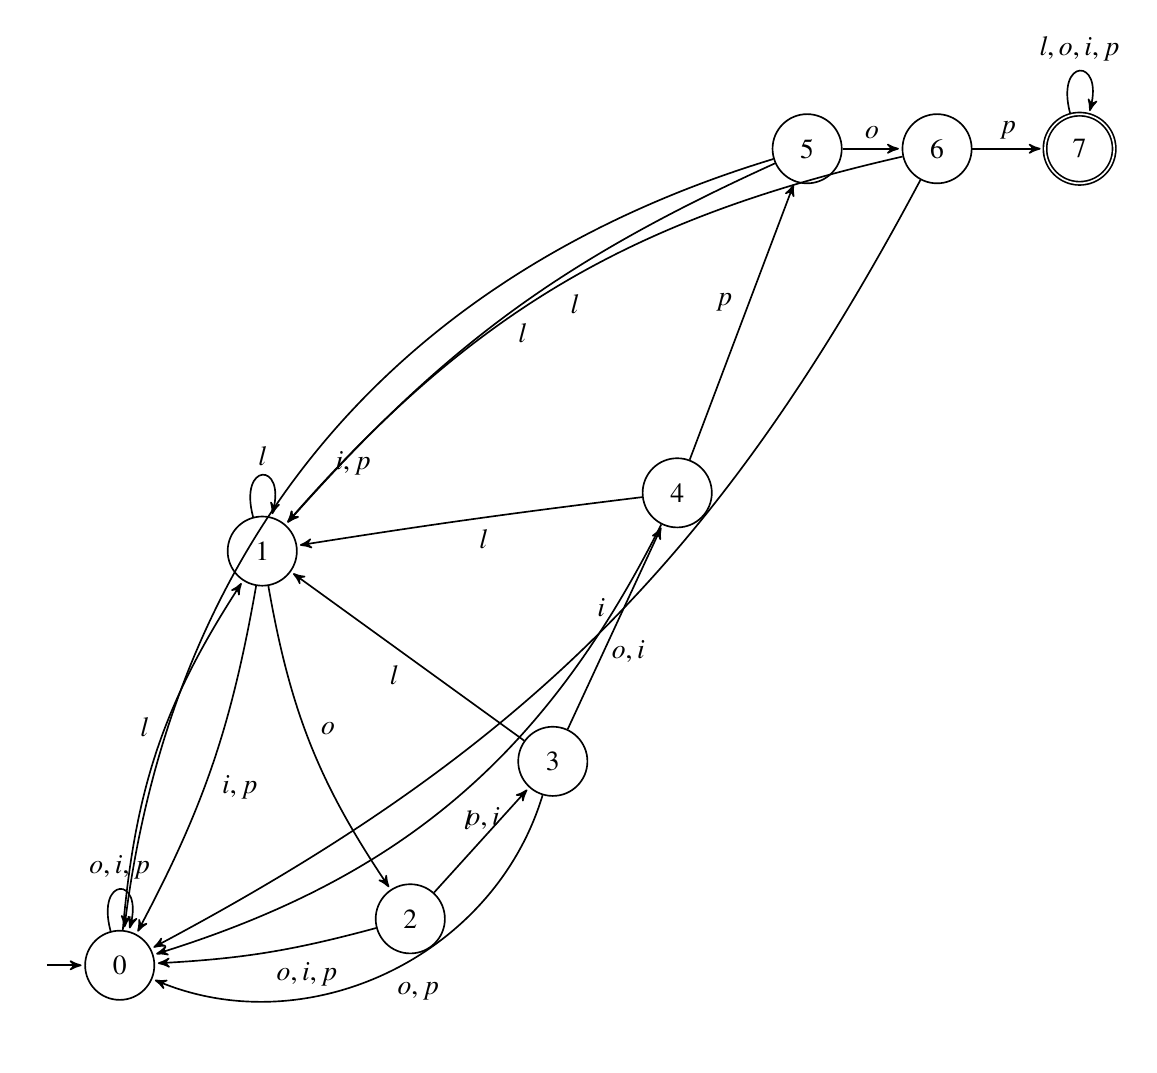
\begin{tikzpicture}[->,>=stealth',shorten >=1pt,auto,node distance=2.8cm,semithick,initial text=$ 	$]
	\node[state, initial, initial where=left] (0) at (2.27,9.41) {$0$};
	\node[state] (1) at (4.08,14.67) {$1$};
	\node[state] (2) at (5.96,10.00) {$2$};
	\node[state] (3) at (7.77,12.00) {$3$};
	\node[state] (4) at (9.35,15.41) {$4$};
	\node[state] (5) at (11.00,19.78) {$5$};
	\node[state] (6) at (12.65,19.78) {$6$};
	\node[state, accepting] (7) at (14.46,19.78) {$7$};
	\path
		(0)

	edge [loop above] node {$o,i,p$} (0)
	edge [bend left = 14] node {$l$} (1)
		(1)

	edge [bend left = 9] node {$i,p$} (0)
	edge [loop above] node {$l$} (1)
	edge [bend right = 12] node {$o$} (2)
		(2)

	edge [bend left = 6] node {$o,i,p$} (0)
	edge node {$l$} (3)
	(3)

	edge [bend left = 48] node {$o,p$} (0)
	edge node {$l$} (1)
	edge node {$i$} (4)
	(4)

	edge [bend left = 23] node {$o,i$} (0)
	edge [bend right = 1] node {$l$} (1)
	edge node {$p$} (5)
	(5)

	edge [bend right = 33] node {$i,p$} (0)
	edge [bend right = 12] node {$l$} (1)
	edge node {$o$} (6)
	(6)

	edge [bend left = 17] node {$o,i$} (0)
	edge [bend right = 18] node {$l$} (1)
	edge node {$p$} (7)
	(7)

	edge [loop above] node {$l,o,i,p$} (7);
\end{tikzpicture}

	%\framebox[\textwidth] {
	%\begin{tikzpicture}[->,>=stealth',shorten >=1pt,auto,node distance=2.8cm,semithick,initial text=$ 	$]
	%	\node[state,initial,initial where=left] (0) at (0,0) {$0$} ;
	%	\node[state] (1) at (12,16) {$1$} ;
	%	\node[state,accepting] (2) at (4,0) {$2$} ;
	%	\node[state] (3) at (0,1) {$3$};
	%	\path
	%		(0)
	%			edge node {$a$} (1)
	%			edge [bend left] node {$b$} (2)
	%		(1)
	%			edge [loop above] node {$a$} (1)
	%			edge [bend left] node {$b$} (0)
	%		(2)
	%			edge [bend left = 10] node {$a$} (0)
	%			edge [loop above] node {$b$} (2);
	%\end{tikzpicture}
	%
	%}
\end{document}